% report.tex
% Scientific article template in English
% Recommended compilation: pdflatex report.tex -> biber report -> pdflatex report.tex (x2)

\documentclass[11pt,a4paper]{article}

% Encoding and language
\usepackage[T1]{fontenc}
\usepackage[utf8]{inputenc}
\usepackage[english]{babel}

% Page layout
\usepackage{geometry}
\geometry{margin=2.5cm}
\usepackage{microtype}

% Graphics, tables, mathematics
\usepackage{graphicx}
\usepackage{booktabs}
\usepackage{amsmath,amssymb,amsthm}
\usepackage{empheq}
\usepackage{siunitx}


% Links, citations
\usepackage[colorlinks=true,linkcolor=blue,citecolor=blue,urlcolor=blue]{hyperref}
\usepackage{csquotes}
% biblatex is loaded later with the desired options to avoid an "Option clash for package biblatex" error

\usepackage[
    backend=biber,
    style=numeric,   % <-- citations sous forme d'entiers
    sorting=none     % pour garder l'ordre d'apparition si tu veux
]{biblatex}

\addbibresource{biblio.bib}

% Useful environments
\theoremstyle{plain}
\newtheorem{theorem}{Theorem}[section]
\theoremstyle{definition}
\newtheorem{definition}{Definition}[section]

% Handy commands
\newcommand{\ie}{\textit{i.e.}}
\newcommand{\eg}{\textit{e.g.}}

% PDF metadata
\hypersetup{
    pdftitle={Automated Calibration of Physical Models for Musical Instruments},
    pdfauthor={Rodolphe Milton VIVANT},
    pdffitwindow=true
}

\title{Automated Calibration of Physical Models for Musical Instruments\\[0.5em]}

\author{Rodolphe Milton VIVANT\thanks{UFR de Mathématique et Informatique de Strasbourg, rodolphe.vivant3@etu-unistra.fr}}
\date{\today}

\begin{document}

\maketitle

\begin{abstract}
Abstract (in English): 
\end{abstract}



\newpage
\section{Introduction}
Present the context, a concise state of the art, the motivation and the main contributions of the paper.

During my project of the thrid semester of the CSMI Master degree, I worked on the automated calibration 
of physical models for musical instruments. 
The goal of this project was to develop a method to automatically adjust the parameters of physical models 
so that they accurately reproduce the sound characteristics of reed instruments. \newline
I worked under the supervision of Dr Emmanuel Franck, Dr Laurent Navoret and Dr Victor Michel-Dansac from 
the Institut de Recherche Mathématique Avancée (IRMA) in Strasbourg and Dr Juliette Chabassier for Modartt. \newline
Modartt \cite{Modartt} is a french company specialized in the development of artistic and technological application softwares.

\subsection{Reed Instruments}
A reed is a thin, flexible lamina mounted at the mouthpiece or at the entrance of an air column resonator that acts \cite{chaigne:hal-05370840} as a valve that controls the airflow driven by a pressure difference between the upstream region 
(the player’s mouth) and the downstream region (the mouthpiece or mouthpiece tip of the instrument). \newline
Two principal categories of reed instruments:
\begin{itemize}
    \item Free reeds (harmonicas, accordions, ...).
    \item Beating reeds (clarinets, saxophones, ...).
\end{itemize}
% Figure : schéma de l'anche / embouchure
\begin{figure}[htbp]
    \centering
    % Remplacez 'figs/reed.png' par le chemin et l'extension réels de votre image (pdf, png, jpg...)
    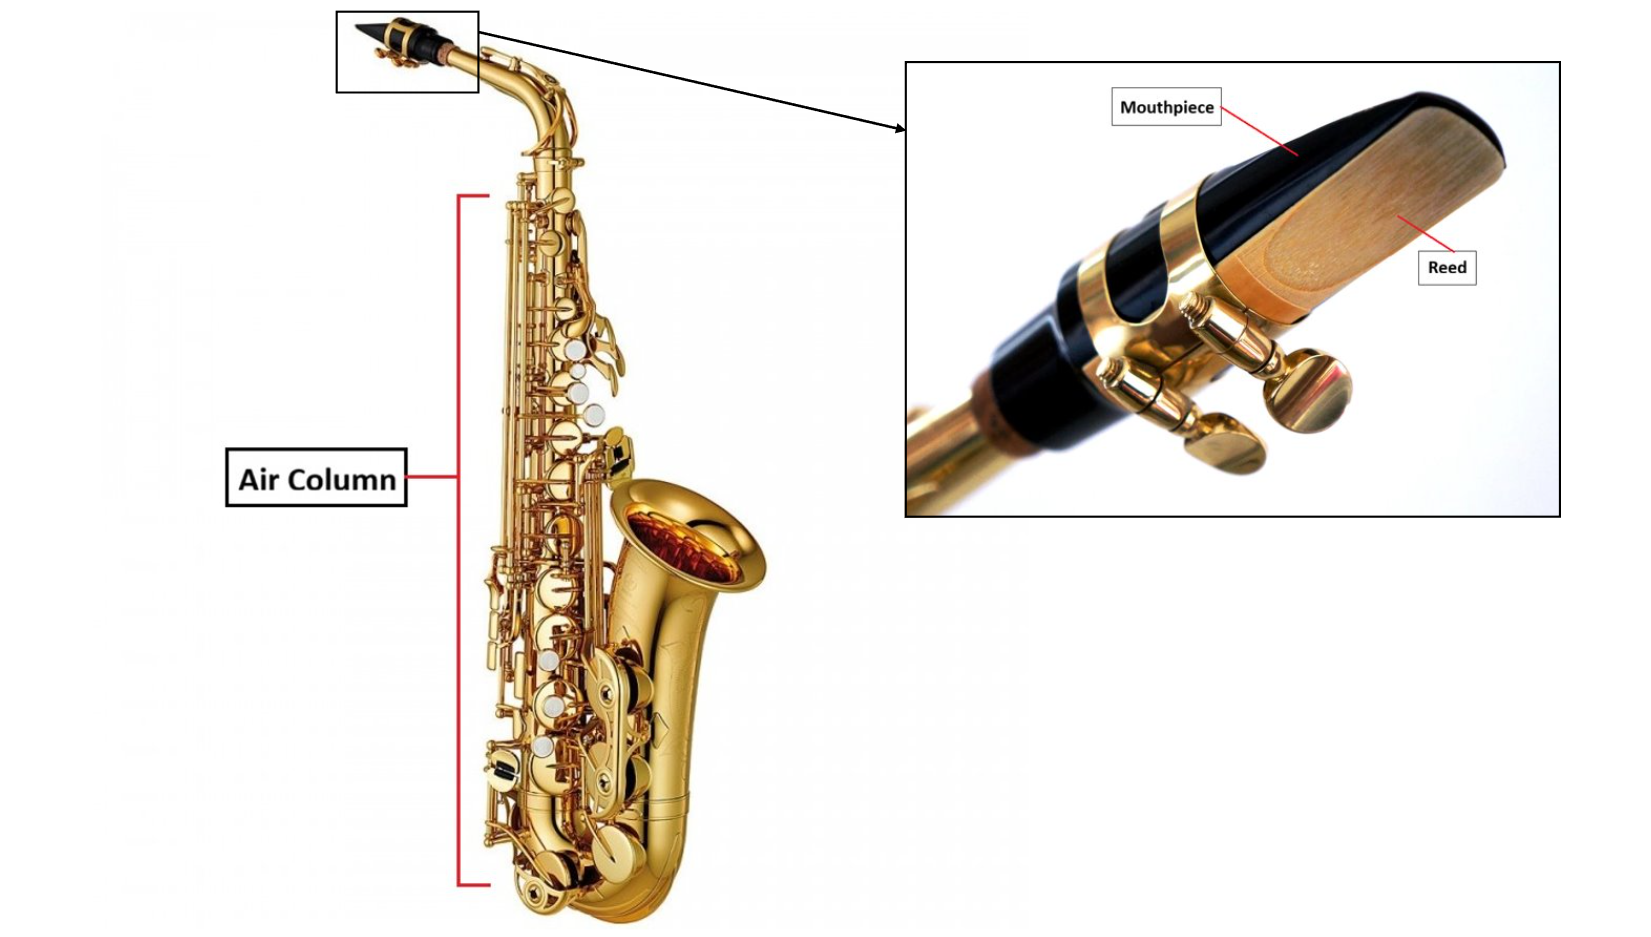
\includegraphics[width=0.9\textwidth]{Images/reed_column.png}
    \caption{Reed and saxophone.}
    \label{fig:reed_schematic}
\end{figure}
\subsection{State of the art}
The equations governing the behavior of reed instruments are mathematically described \cite{MAMAMIA2024} by a set of coupled 
differential equations (Partial Differential Equations - PDEs, Ordinary Differential Equations - ODEs, and 
algebraic equations). These equations capture the complex interactions between the pressure ($p$), the acoustic
volume velocity ($v$) \eqref{eq:1a} \eqref{eq:1b}, some radiative phenomenons ($\phi$) \eqref{eq:1c} \eqref{eq:1d}, 
and the effects of the instrumental player \eqref{eq:1e} \eqref{eq:1f} :
% Système d'équations décrivant un modèle réducteur pour un instrument à anche
\begin{subequations}
\begin{empheq}[left=\empheqlbrace]{align}
  \frac{S(x)}{c S^\ast}\,\partial_t p(x,t) + \partial_x v(x,t) &= 0 \label{eq:1a}\\[4pt]
  \frac{S^\ast}{c S(x)}\,\partial_t v(x,t) + \partial_x p(x,t) &= 0 \label{eq:1b}\\[4pt]
  \frac{Z^\ast}{T}\,\partial_t \phi + \sqrt{\alpha}\,p(L,t) &= 0 \label{eq:1c}\\[4pt]
  -\frac{\beta}{Z^\ast T}\,p(L,t) + v(L,t) + \sqrt{\alpha}\,\phi &= 0 \label{eq:1d}\\[4pt]
  -v(0,t) + \zeta_\ell(y)\,F(\gamma - p(0,t)) + \varepsilon\frac{\kappa}{\omega_r}\,\partial_t y &= 0 \label{eq:1e}\\[6pt]
  \frac{1}{\omega_r^2}\,\partial_{tt} y + \frac{1}{Q_r\omega_r}\,\partial_t y + y - 1 
  &= \varepsilon(\gamma - p(0,t)) \label{eq:1f}
\end{empheq}
\end{subequations}

where $S(x)$ is the cross-sectional area of the instrument at position $x$, $S^\ast$ is a reference area,
$c$ is the speed of sound, $Z^\ast$ is a reference acoustic impedance, $T$ is a characteristic time, 
$\alpha$ and $\beta$ are parameters related to the radiation effects, $L$ is the length of the instrument,
$\zeta_\ell(y)$ is a function representing the lip-reed coupling, $F$ is a nonlinear function ($F(\Delta p)=\Delta p \, \text{sign} (\Delta p)$),
$\gamma$ is the dimensionless blowing pressure, $\varepsilon$ =-1 for a reed instrument, 
$\kappa$ is a parameter related to the lip dynamics, $\omega_r$ is the reed's (or lips') frequency ($=2\pi f_r$), 
$Q_r$ is the quality factor of the reed, and $y$ is the dimensionless reed opening. \newline
This kind of system of equation can already be solved numerically with Openwind \cite{OpenwindInria}.

\subsection{Objectives}
The main objectives of this project were:
In JAX framework:
\begin{enumerate}
    \item Implement a discontinous Galerkin discretization of the mixed form of the wave equation and numerically solve it.
    \item Implement the coupling with an ODE and the boundary conditions.
    \item Compute the gradient with respect to all the problem parameters.   
\end{enumerate}

\section{Methods}
Describe the method, model or algorithm. Include the essential equations.
\subsection{Discontinuous Galerkin Method \cite{HesthavenWarburton2008}}

The Discontinuous Galerkin Method (DGM) is a numerical technique used to solve partial differential equations (PDEs). 
Let's consider an equation of the form :
\begin{equation}
    \frac{\partial u}{\partial t} + \frac{\partial F(u)}{\partial x} = 0,
\end{equation}
where $u(x,t)$ is the unknown function and $F(u)$ is a flux function. \newline
The DGM involves the following steps:
\begin{enumerate}
    \item \textbf{Domain Discretization:} Divide the spatial domain into a finite number of elements or cells.
    \item \textbf{Basis Functions:} Choose a set of basis functions (often polynomials) to represent the solution within each element.
    \item  \textbf{Weak Formulation:} Multiply the PDE by a test function (which can be one of the basis functions) and integrate over each element to obtain the weak form of the equation.
    \item \textbf{Numerical Fluxes:} Define numerical fluxes at the interfaces between elements to ensure stability and consistency.
    \item \textbf{Time Integration:} Use an appropriate time-stepping method (e.g., Runge-Kutta) to advance the solution in time.
\end{enumerate} 

Let's denote the approximate solution at the $n$-th time step as $u^n(x)$. The update from time step $n$ to $n+1$ can be expressed as:
\begin{equation}
    u^{n+1}(x) = u^n(x) - \Delta t \partial_x F(u^n)
\end{equation}

Let's consider test function $\phi_i(x)$, the weak form of the equation becomes in a one cell $\Omega_k$:
\begin{equation}
    \int_{\Omega_k} \phi_i(x)  u^{n+1} \, dx =  \int_{\Omega_k} \phi_i(x)  u^{n} \, dx - \Delta t \int_{\Omega_k} \phi_i(x) \partial _x F(u^n) \, dx
\end{equation}
Using integration by parts on the second term, we get:
\begin{equation}
    \int_{\Omega_k} \phi_i(x)  u^{n+1} \, dx =  \int_{\Omega_k} \phi_i(x)  u^{n} \, dx + \Delta t \int_{\Omega_k} \partial_x \phi_i(x) F(u^n) \, dx - \Delta t \left[ \phi_i(x) F(u^n) \right]_{\partial \Omega_k}
\end{equation}
where $\left[ \phi_i(x) F(u^n) \right]_{\partial \Omega_k}$ represents the numerical flux at the boundaries of the element $\Omega_k$.

Finally, by expressing $u^{n+1} = \sum_j \alpha_{k,j} \phi_j(x)$ within each element, we can derive a system of equations for the coefficients $\alpha_{k,j}$ that can be solved at each time step :
\begin{equation}
    \sum_j \alpha_{k,j}^{n+1} \int_{\Omega_k} \phi_i(x) \phi_j(x) \, dx = \int_{\Omega_k} \phi_i(x)  u^{n} \, dx + \Delta t \int_{\Omega_k} \partial_x \phi_i(x) F(u^n) \, dx - \Delta t \left[ \phi_i(x) F(u^n) \right]_{\partial \Omega_k}
\end{equation}

where $M_{ij} = \int_{\Omega_k} \phi_i(x) \phi_j(x) \, dx$ is a component of the local mass matrix $M$.

And so finally we can write the update rule for the coefficients $\alpha_{k,j}$ as:
\begin{equation}
    M\alpha_{k}^{n+1} = b_k
\end{equation}
where $b_k$ is the right-hand side vector containing the integrals and numerical fluxes.

\subsection{Discontinuous Galerkin in our context}

\subsubsection{Conservative form}
In our case, we are interested in solving the mixed form of the wave equation given by the system {\eqref{eq:1a}--\eqref{eq:1b}}. We can rewrite this system in vector form as:
\begin{equation}
\mathbf{C}(x)\partial_t \mathbf{u} +\partial_x \mathbf{A}\mathbf{u} = 0
\end{equation}

where $\mathbf{u} = \begin{pmatrix} p \\ v \end{pmatrix}$,$\mathbf{C}=\begin{pmatrix} \frac{S(x)}{cS^*} & 0 \\ 0 & \frac{S^*}{S(x)c} \end{pmatrix}$ $\mathbf{A} = \begin{pmatrix} 0 & 1 \\ 1 & 0 \end{pmatrix}$. \newline
and the initial condition : $p(x,0) = p_0(x)$ and $v(x,0) = v_0(x)$ \newline

\subsubsection{Mesh and DG space}
For a mesh
$$
0 = x_0 < x_1 < ... < x_{N} = L; \quad K_j=(x_{j-1}, x_j), \quad j=1,...,N
$$
We are searching a approched solution  $\mathbf{u_h} = (p_h, v_h)^T \in (V_h^k)^2$ with $V_h^k=\{u\in L^2 : u|_{K_j} \in \mathbb{P}^1{K_j}\}$ 

\subsubsection{Local DG Formulation}
For each element $K_j$ and for each test function vector $\mathbf{\Phi}=(\phi_p,\phi_v)^T \in (\mathbb{P}^1{K_j})^2$, we have the following weak formulation :

\begin{equation}
    \begin{aligned}
\int_{K_j} \mathbf C(x)\, \partial_t \mathbf u_h \cdot \mathbf \Phi \, dx
-
\int_{K_j} \mathbf A\, \mathbf u_h \cdot \partial_x \mathbf \Phi \, dx
& \\
\quad
+ \widehat{\mathbf F}_{j+\frac12} \cdot \mathbf \Phi(x_j^-)
-
\widehat{\mathbf F}_{j-\frac12} \cdot \mathbf \Phi(x_{j-1}^+)
&= 0.
\end{aligned}
\end{equation}
where $\mathbf{F}(\mathbf{u})=\mathbf{AU} = \begin{pmatrix} v \\ p \end{pmatrix}$ 

\subsubsection{RusanovFlux}
At each interface $x_{j+\frac12}$, the Rusanov numerical flux:
(Local Lax--Friedrichs) is defined by
\begin{equation}
\widehat{\mathbf F}
=
\frac12\Big(
\mathbf F(\mathbf u^-)
+
\mathbf F(\mathbf u^+)
\Big)
-
\frac{\lambda_{j+\frac12}}{2}
\Big(
\mathbf u^+ - \mathbf u^-
\Big),
\end{equation}
où
$
\lambda_{j+\frac12}
=
\max\bigl(|\lambda_1|,|\lambda_2|\bigr).
$

The eighen values $\lambda_1, \lambda_2$ of the matrix $\mathbf{C}^{-1}\mathbf{A}$ are :
$$
\lambda_{1,2}
=
\pm c.
$$

Therefore, for the Rusanov flux, we have :
$$
\lambda_{j+\frac12}=c.
$$

\subsubsection{Explicit flux}
By denoting
$$
\mathbf U^\pm =
\begin{pmatrix}
p^\pm\\
v^\pm
\end{pmatrix},
\qquad
\mathbf F(\mathbf U)=
\begin{pmatrix}
v\\
p
\end{pmatrix},
$$
The numerical flux at each interface is given by :
$$
\widehat{\mathbf F} =
\begin{pmatrix}
\widehat{v}\\
\widehat{p}
\end{pmatrix},
$$
with
$$
\boxed{
\begin{aligned}
\widehat{v}
& =
\frac12\left(v^-+v^+\right)
-
\frac{c}{2}\left(p^+-p^-\right),
\\
\widehat{p}
& =
\frac12\left(p^-+p^+\right)
-
\frac{c}{2}\left(v^+-v^-\right).
\end{aligned}
}
$$

\subsubsection{Final DG formulation}
For each element $K_j=(x_{j-1},x_j)$ and 
for each test function $w_p,w_v\in\mathbb P^k(K_j)$, 
the DG formulation of the mixed form of the wave equation reads :

\begin{equation}
\begin{aligned}
\int_{K_j} \frac{S(x)}{cS^\ast}\,
\partial_t p_h \, \phi_p \, dx
&-
\int_{K_j} v_h \, \partial_x \phi_p \, dx \\
&+
\widehat{v}_{j+\frac12}\, \phi_p(x_j^-)
-
\widehat{v}_{j-\frac12}\, \phi_p(x_{j-1}^+)
=0,
\end{aligned}
\label{eq:dg_wave_p}
\end{equation}

\begin{equation}
\begin{aligned}
\int_{K_j} \frac{S^\ast}{cS(x)}\,
\partial_t v_h \, \phi_v \, dx
&-
\int_{K_j} p_h \, \partial_x \phi_v \, dx \\
&+
\widehat{p}_{j+\frac12}\, \phi_v(x_j^-)
-
\widehat{p}_{j-\frac12}\, \phi_v(x_{j-1}^+)
=0.
\end{aligned}
\label{eq:dg_wave_v}
\end{equation}
All the dependence on the variable cross-sectional area $S(x)$ is contained in the mass matrix C(x). 
This property ensures a uniform wave speed c and a CFL condition independent of S(x)
\subsubsection{Boundary conditions}

On the righthand-side boundary ($x=L$), we need to ensure the conditions derived from equations {\eqref{eq:1c}--\eqref{eq:1d}}.

\begin{equation}
v(L,t) = \frac{\beta}{Z_T^*} p(L,t) - \sqrt{\alpha}\,\phi(t).
\tag{BC}
\end{equation}

From the characteristic variables defined as :
\begin{equation}
w^+ = p + v,
\qquad
w^- = p - v.
\end{equation}

At the right boundary, the wave $\omega^+$ is outgoing while $\omega^-$ is incoming.
The boundary condition must therefore provide a relation to determine $w^-$.

From the definition of $w^-$ and the boundary condition (BC), we have:
\begin{equation}
    \begin{aligned}
        w^-
        &= p - v \\
        &= p - \left( \frac{\beta}{Z_T^*} p - \sqrt{\alpha},\phi \right) \\
        &= \left(1 - \frac{\beta}{Z_T^*}\right)p + \sqrt{\alpha},\phi.
    \end{aligned}
\end{equation}

And the expression of $p$ in terms of $w^+$ and $w
^-$ is :
\begin{equation}
p = \frac{w^+ + w^-}{2}.
\end{equation}

By substituting this into the previous equation, we obtain:
\begin{equation}
w^-
= \left(1 - \frac{\beta}{Z_T^*}\right)\frac{w^+ + w^-}{2} + \sqrt{\alpha} \phi.
\end{equation}

So the incoming wave $w^-$ can be expressed as:
\begin{equation}
\boxed{
w^- =
\frac{1 - \frac{\beta}{Z_T^*}}{1 + \frac{\beta}{Z_T^*}}
w^+
+
\frac{2\sqrt{\alpha}}{1 + \frac{\beta}{Z_T^*}} \phi
}
\end{equation}

\subsection{Analytical solving when $S(x) = S^* = 1$}
To assess the validity of our Discontinuous Galerkin Method implementation, we can compare the numerical solution to the analytical solution in the simple case where $S(x) = S^* = 1$.
Let's consider the following equation system :
\begin{align}
    \partial_t p + c\,\partial_x v &= 0, \\
    \partial_t v + c\,\partial_x p &= 0.
\end{align}
with the boundary conditions {\eqref{eq:1c}--\eqref{eq:1d}}. 
\subsubsection{Riemann invariants}
Introduce the Riemann variables
\begin{equation}
    r := p+v,\qquad s := p-v.
\end{equation}
They satisfy decoupled transport equations
\begin{align}
    \partial_t r + c\,\partial_x r &= 0, \label{eq:transport_r}\\
    \partial_t s - c\,\partial_x s &= 0. \label{eq:transport_s}
\end{align}
With initial data $p(x,0)=p_0(x)$, $v(x,0)=v_0(x)$ we have $r_0=p_0+v_0$ and $s_0=p_0-v_0$, hence from \eqref{eq:transport_r}--\eqref{eq:transport_s}
\begin{equation}
    r(x,t)=r_0(x-ct),\qquad s(x,t)=s_0(x+ct).
\end{equation}
Recovering $(p,v)$ gives the explicit solution
\begin{align}
    p(x,t) &= \tfrac12\bigl[r_0(x-ct)+s_0(x+ct)\bigr] \nonumber\\
                 &= \tfrac12\bigl[p_0(x-ct)+p_0(x+ct)\bigr] 
                        + \tfrac12\bigl[v_0(x-ct)-v_0(x+ct)\bigr] \label{eq:solution_p}, \\
    v(x,t) &= \tfrac12\bigl[r_0(x-ct)-s_0(x+ct)\bigr] \nonumber\\
                 &= \tfrac12\bigl[v_0(x-ct)+v_0(x+ct)\bigr] 
                        + \tfrac12\bigl[p_0(x-ct)-p_0(x+ct)\bigr] \label{eq:solution_v}.
\end{align}
\subsubsection{Boundary condition at $x=L$}

At the right boundary $x=L$, we impose a dynamic impedance-type boundary condition
coupled with an auxiliary variable $\phi(t)$:
\begin{align}
&\partial_t \phi(t) + c_1\,r(L,t) + c_2\,\phi(t) = 0, \label{eq:phi_bc} \\
&s(L,t) = a\,r(L,t) + b\,\phi(t), \label{eq:s_bc}
\end{align}
where the coefficients are given by
\begin{equation}
a=\frac{1-\beta/Z_T}{1+\beta/Z_T}, \qquad
b=\frac{2\sqrt{\alpha}}{1+\beta/Z_T}, \qquad
c_1=\frac{\sqrt{\alpha}}{2Z_T}, \qquad
c_2=c_1 b. \label{eq:coeffs}
\end{equation}

The incoming characteristic at the boundary is
\begin{equation}
r(L,t)=p_0(L-ct), \label{eq:r_boundary}
\end{equation}
while the outgoing characteristic $s(L,t)$ is determined by
\eqref{eq:s_bc}--\eqref{eq:phi_bc}.  
This ordinary differential equation system is solved explicitly in time and then propagated
into the domain along characteristics.

\subsubsection{Final analytical solution}

Denoting by $s_{\mathrm{ref}}(x,t)$ the reflected wave generated at $x=L$ and transported
with velocity $-c$, the total right-going characteristic reads
\begin{equation}
s(x,t)=p_0(x+ct)+s_{\mathrm{ref}}(x,t),
\end{equation}
while the left-going characteristic remains
\begin{equation}
r(x,t)=p_0(x-ct).
\end{equation}

The pressure and velocity fields are finally reconstructed as
\begin{align}
p(x,t) &= \frac12\bigl[r(x,t)+s(x,t)\bigr], \label{eq:p_final} \\
v(x,t) &= \frac12\bigl[r(x,t)-s(x,t)\bigr]. \label{eq:v_final}
\end{align}

This analytical solution is exactly the one implemented in the function
\texttt{exact\_solution\_characteristics} and is used as a reference to assess the accuracy
of the DG scheme.

\section{Numerical Results}

\subsection{Initial Condition}
The initial pressure profile is defined as a smooth compactly supported bump function
centered at $x=L/2$. Introducing the rescaled variable
\begin{equation}
\xi(x) = \frac{4}{L}\left(x - \frac{L}{2}\right),
\end{equation}
the initial condition reads
\begin{equation}
p_0(x) =
\begin{cases}
\dfrac{\phi_0}{4}\,
\exp\!\left(1 - \dfrac{1}{1-\xi(x)^2}\right),
& \text{if } |\xi(x)| < 1, \\[1.2ex]
0, & \text{otherwise}.
\end{cases}
\end{equation}

The initial acoustic volume velocity is set to zero:
\begin{equation}
v_0(x) = 0.
\end{equation}

\newpage
\subsection{DG Method results}

\subsubsection{Uniform cross-section}

In the case of a uniform cross-section $S(x) = S^* = 1$, the analytical solution described in \eqref{eq:solution_p}--\eqref{eq:solution_v} is available for validation.

\paragraph{Solution plots} $\\ \\$

\begin{figure}[htbp]
    \centering
    % Remplacez 'figs/dg_solution.png' par le chemin et l'extension réels de votre image (pdf, png, jpg...)
    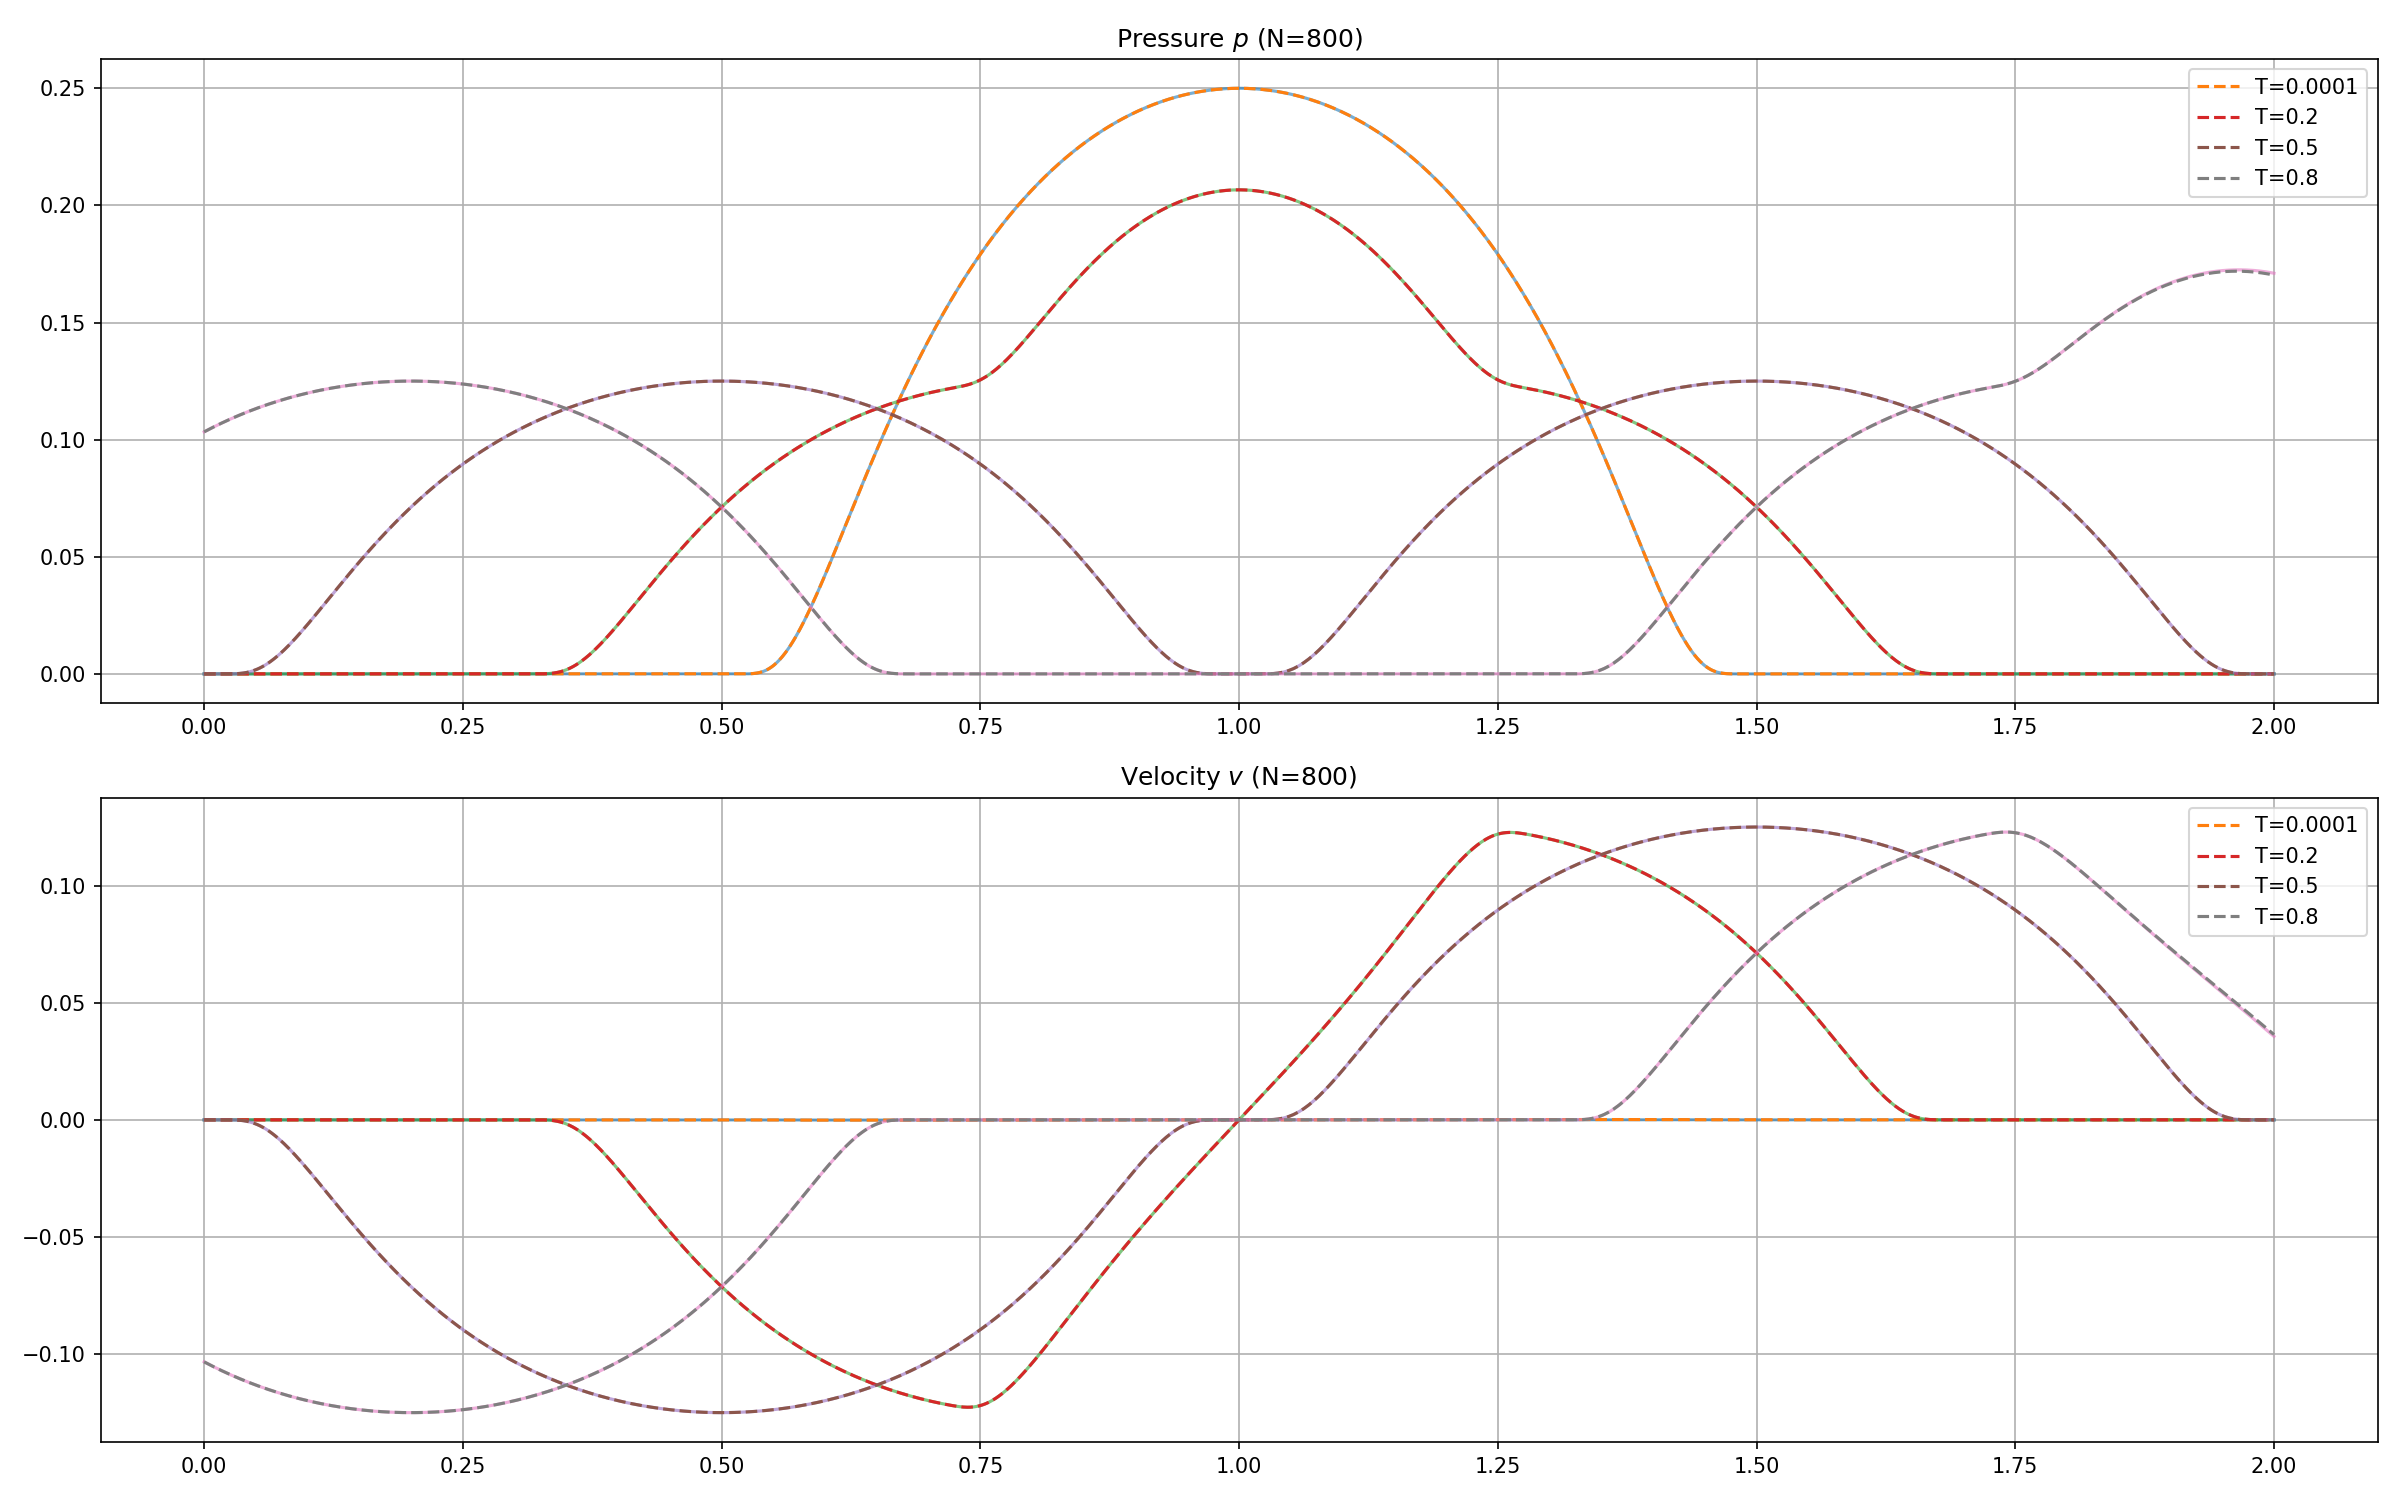
\includegraphics[width=0.9\textwidth]{Images/dg_solution_const_N800.png}
    \caption{DG numerical solutions constant cross-section.}
    \label{fig:dg_solution_const}
\end{figure}

As shown in Figure \ref{fig:dg_solution_const}, the numerical solution obtained using the Discontinuous Galerkin Method accurately captures 
the wave propagation over time described in \ref{eq:solution_p} and \ref{eq:solution_v}. The method effectively resolves the wave fronts 
and maintains stability throughout the simulation.
Inside the domain (Instrument), we can observe the proper propagation of the initial pressure bump, splitting into left-going and right-going waves for the pressure 
and velocity fields. At the right boundary, the interaction with the radiation condition seems to be correctly
computed hence demonstrating the method's capability to handle complex boundary conditions.

\paragraph{Convergence study} $\\ \\$ 
The convergence of the DG method is verified by comparing the numerical solution to the analytical solution at various size of discrectisation with an Explicit Euler
time integration scheme and a Runge-Kutta 2nd order scheme. 
\newpage
\begin{figure}[htbp]
    \centering
    \begin{minipage}[t]{0.48\textwidth}
        \centering
        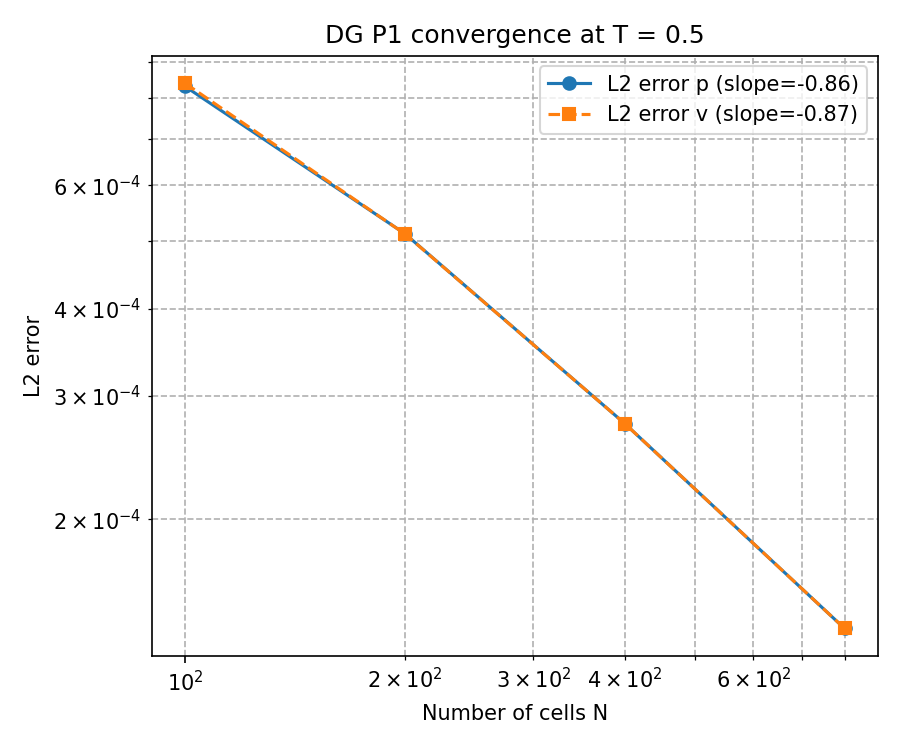
\includegraphics[width=\textwidth]{Images/dg_convergence_T0p5_euler.png}
        \caption{Convergence of the DG method with Explicit Euler scheme.}
        \label{fig:convergence_plot_euler}
    \end{minipage}
    \hfill
    \begin{minipage}[t]{0.48\textwidth}
        \centering
        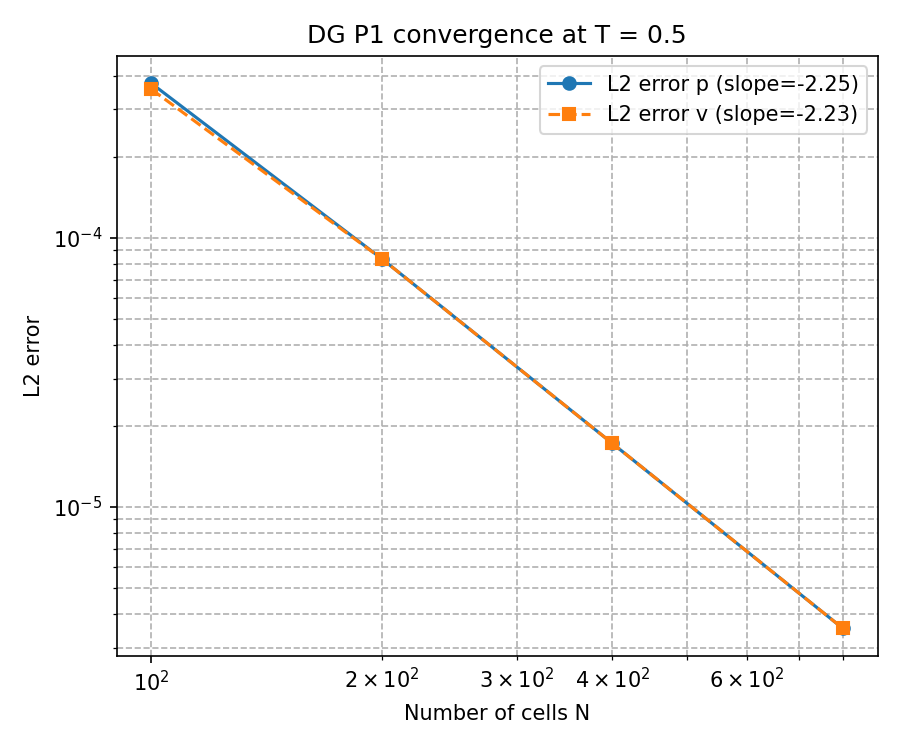
\includegraphics[width=\textwidth]{Images/dg_convergence_T0p5_rk2.png}
        \caption{Convergence of the DG method with Rk2 scheme.}
        \label{fig:convergence_plot_rk2}
    \end{minipage}
\end{figure}

The numerical results confirm the theoretical convergence rates of the discontinuous Galerkin method.
For a polynomial degree $d$, the spatial discretization achieves an order of accuracy
$\mathcal{O}(h^{d+1})$ in the $L^2$ norm for sufficiently smooth solutions.
The overall convergence rate of the fully discrete scheme is 
limited by the order of the time integration method: first order for 
the explicit Euler scheme and second order for the second-order 
Runge–Kutta scheme.

\subsubsection{Non-uniform cross-section}
In the case of a non-uniform cross-section $S(x) \neq S^*$, no analytical solution is available.
\paragraph{Case of an exponential cross-section} $\\ \\$
We consider an exponential cross-section defined as
\begin{figure}[htbp]
    \centering
    \begin{minipage}[c]{0.4\textwidth}
        \centering
        \vfill
        \begin{equation}
            S(x) = S_0 \exp(k x)
        \end{equation}
        where $S_0 > 0$ and $k$ are given constants.
        \vfill
    \end{minipage}
    \hfill
    \begin{minipage}[c]{0.58\textwidth}
        \centering
        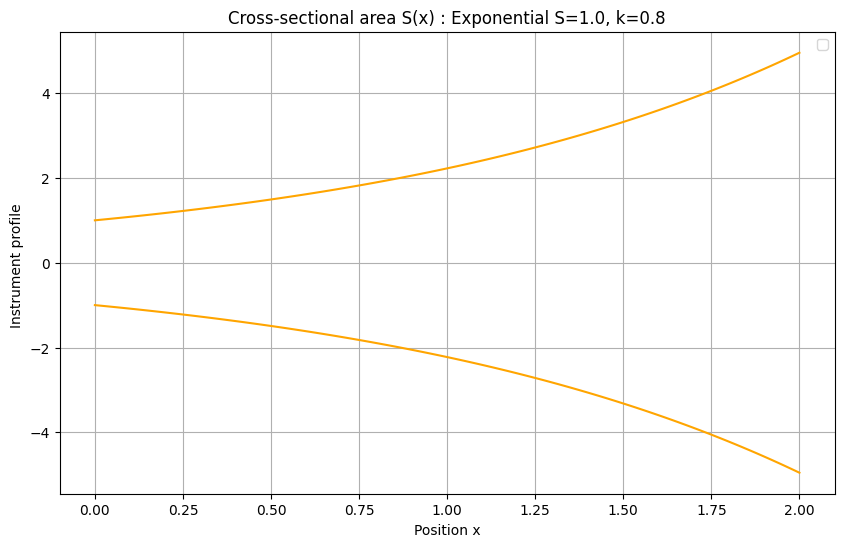
\includegraphics[width=\textwidth]{Images/exp_profile.png}
    \end{minipage}
    \caption{Exponential variation of the cross-sectional area $S(x)$.}
    \label{fig:exp_profile}
\end{figure}

This is the shape of the clarinet bell for example.

\begin{figure}[htbp]
    \centering
    % Remplacez 'figs/dg_solution.png' par le chemin et l'extension réels de votre image (pdf, png, jpg...)
    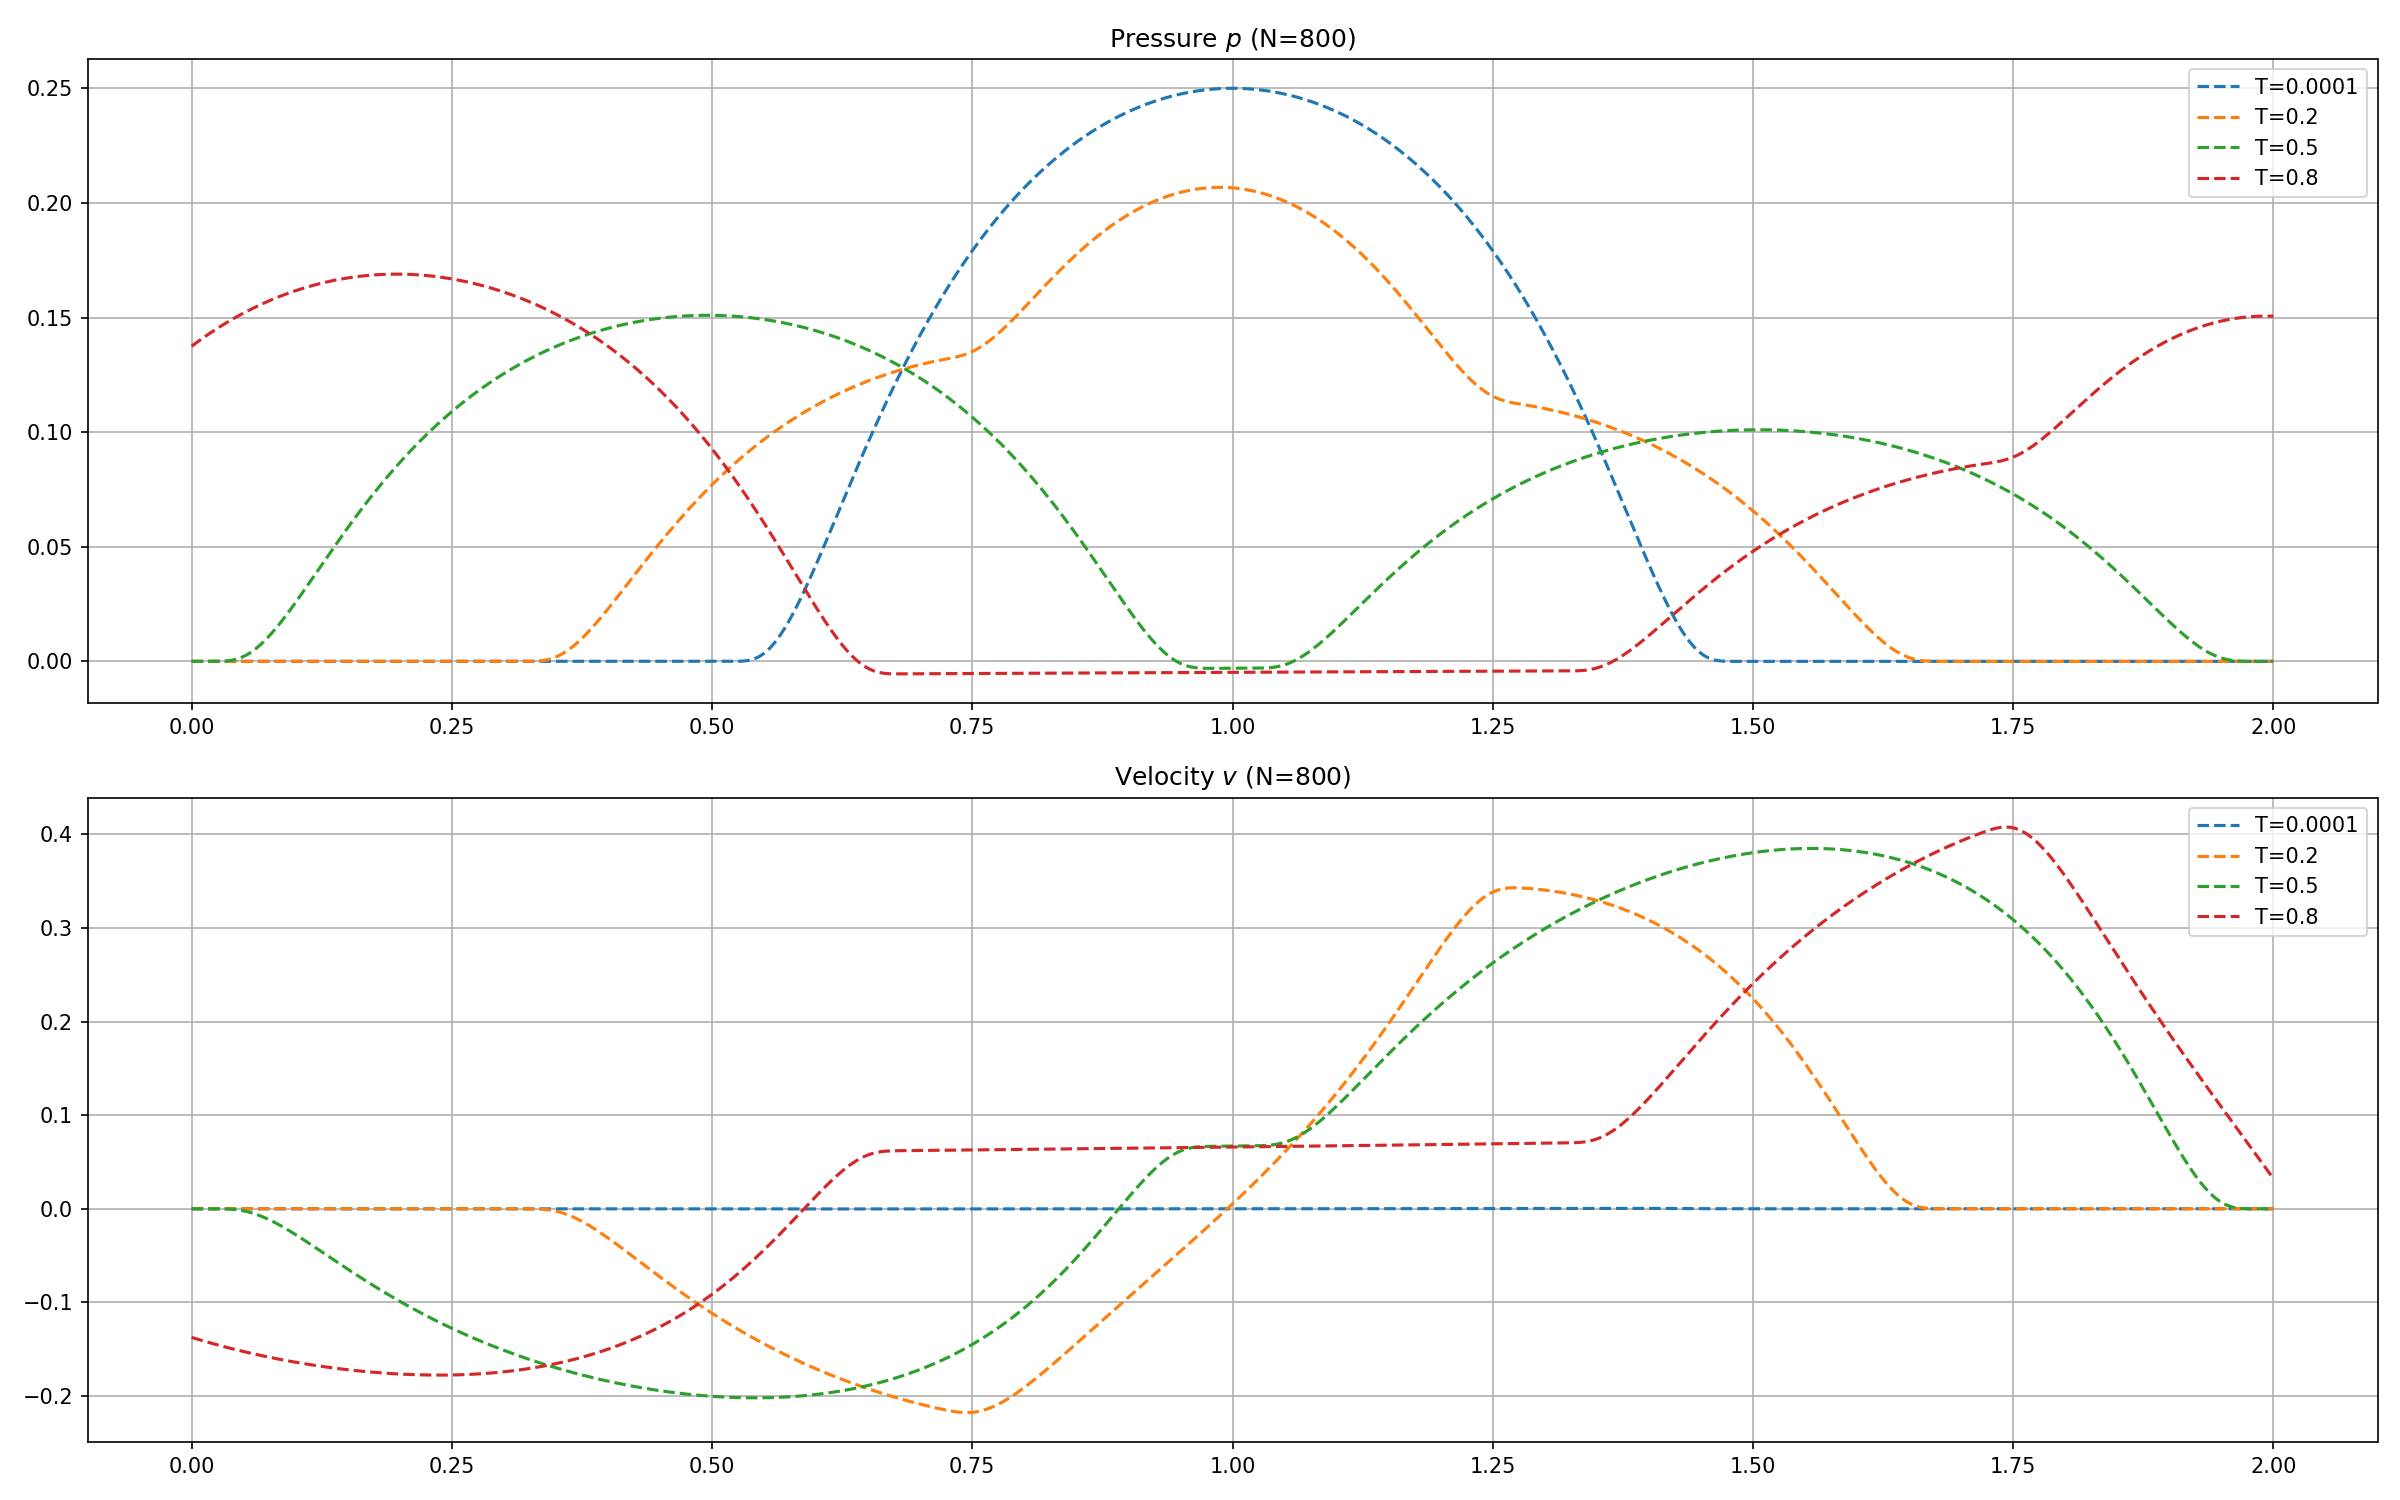
\includegraphics[width=0.9\textwidth]{Images/dg_solution_exp_N800.png}
    \caption{DG numerical solutions exponential cross-section.}
    \label{fig:dg_solution_exp}
\end{figure}

\newpage
\paragraph{Case of a conical cross-section} $\\ \\$
We consider a conical cross-section defined as
\begin{figure}[htbp]
    \centering
    \begin{minipage}[c]{0.4\textwidth}
        \centering
        \vfill
        \begin{equation}
            S(x) = S_0 + k x
        \end{equation}
        where $S_0 > 0$ and $k$ are given constants.
        \vfill
    \end{minipage}
    \hfill
    \begin{minipage}[c]{0.58\textwidth}
        \centering
        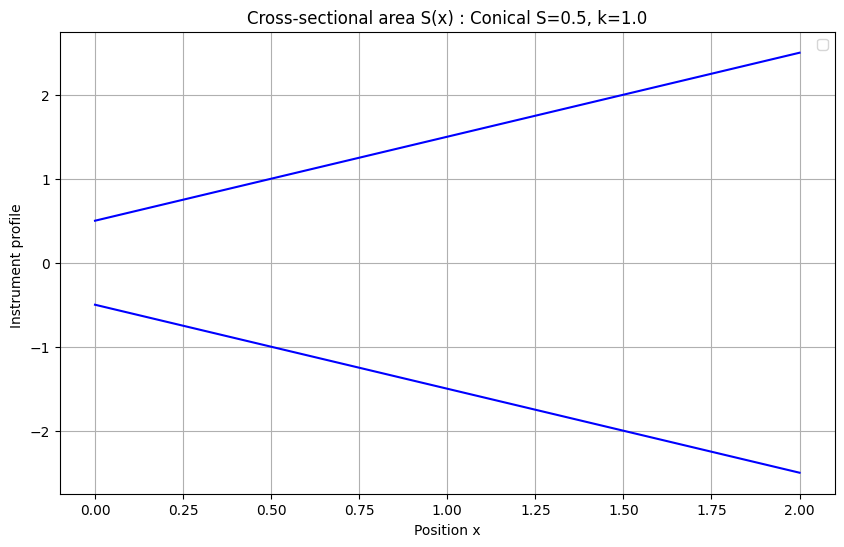
\includegraphics[width=0.9\textwidth]{Images/cone_profile.png}
    \end{minipage}
    \caption{Profile of an instrument with a conical cross-section.}
    \label{fig:cone_profile}
\end{figure}

This is another shape of musical instrument.

\newpage
\begin{figure}[htbp]
    \centering
    % Remplacez 'figs/dg_solution.png' par le chemin et l'extension réels de votre image (pdf, png, jpg...)
    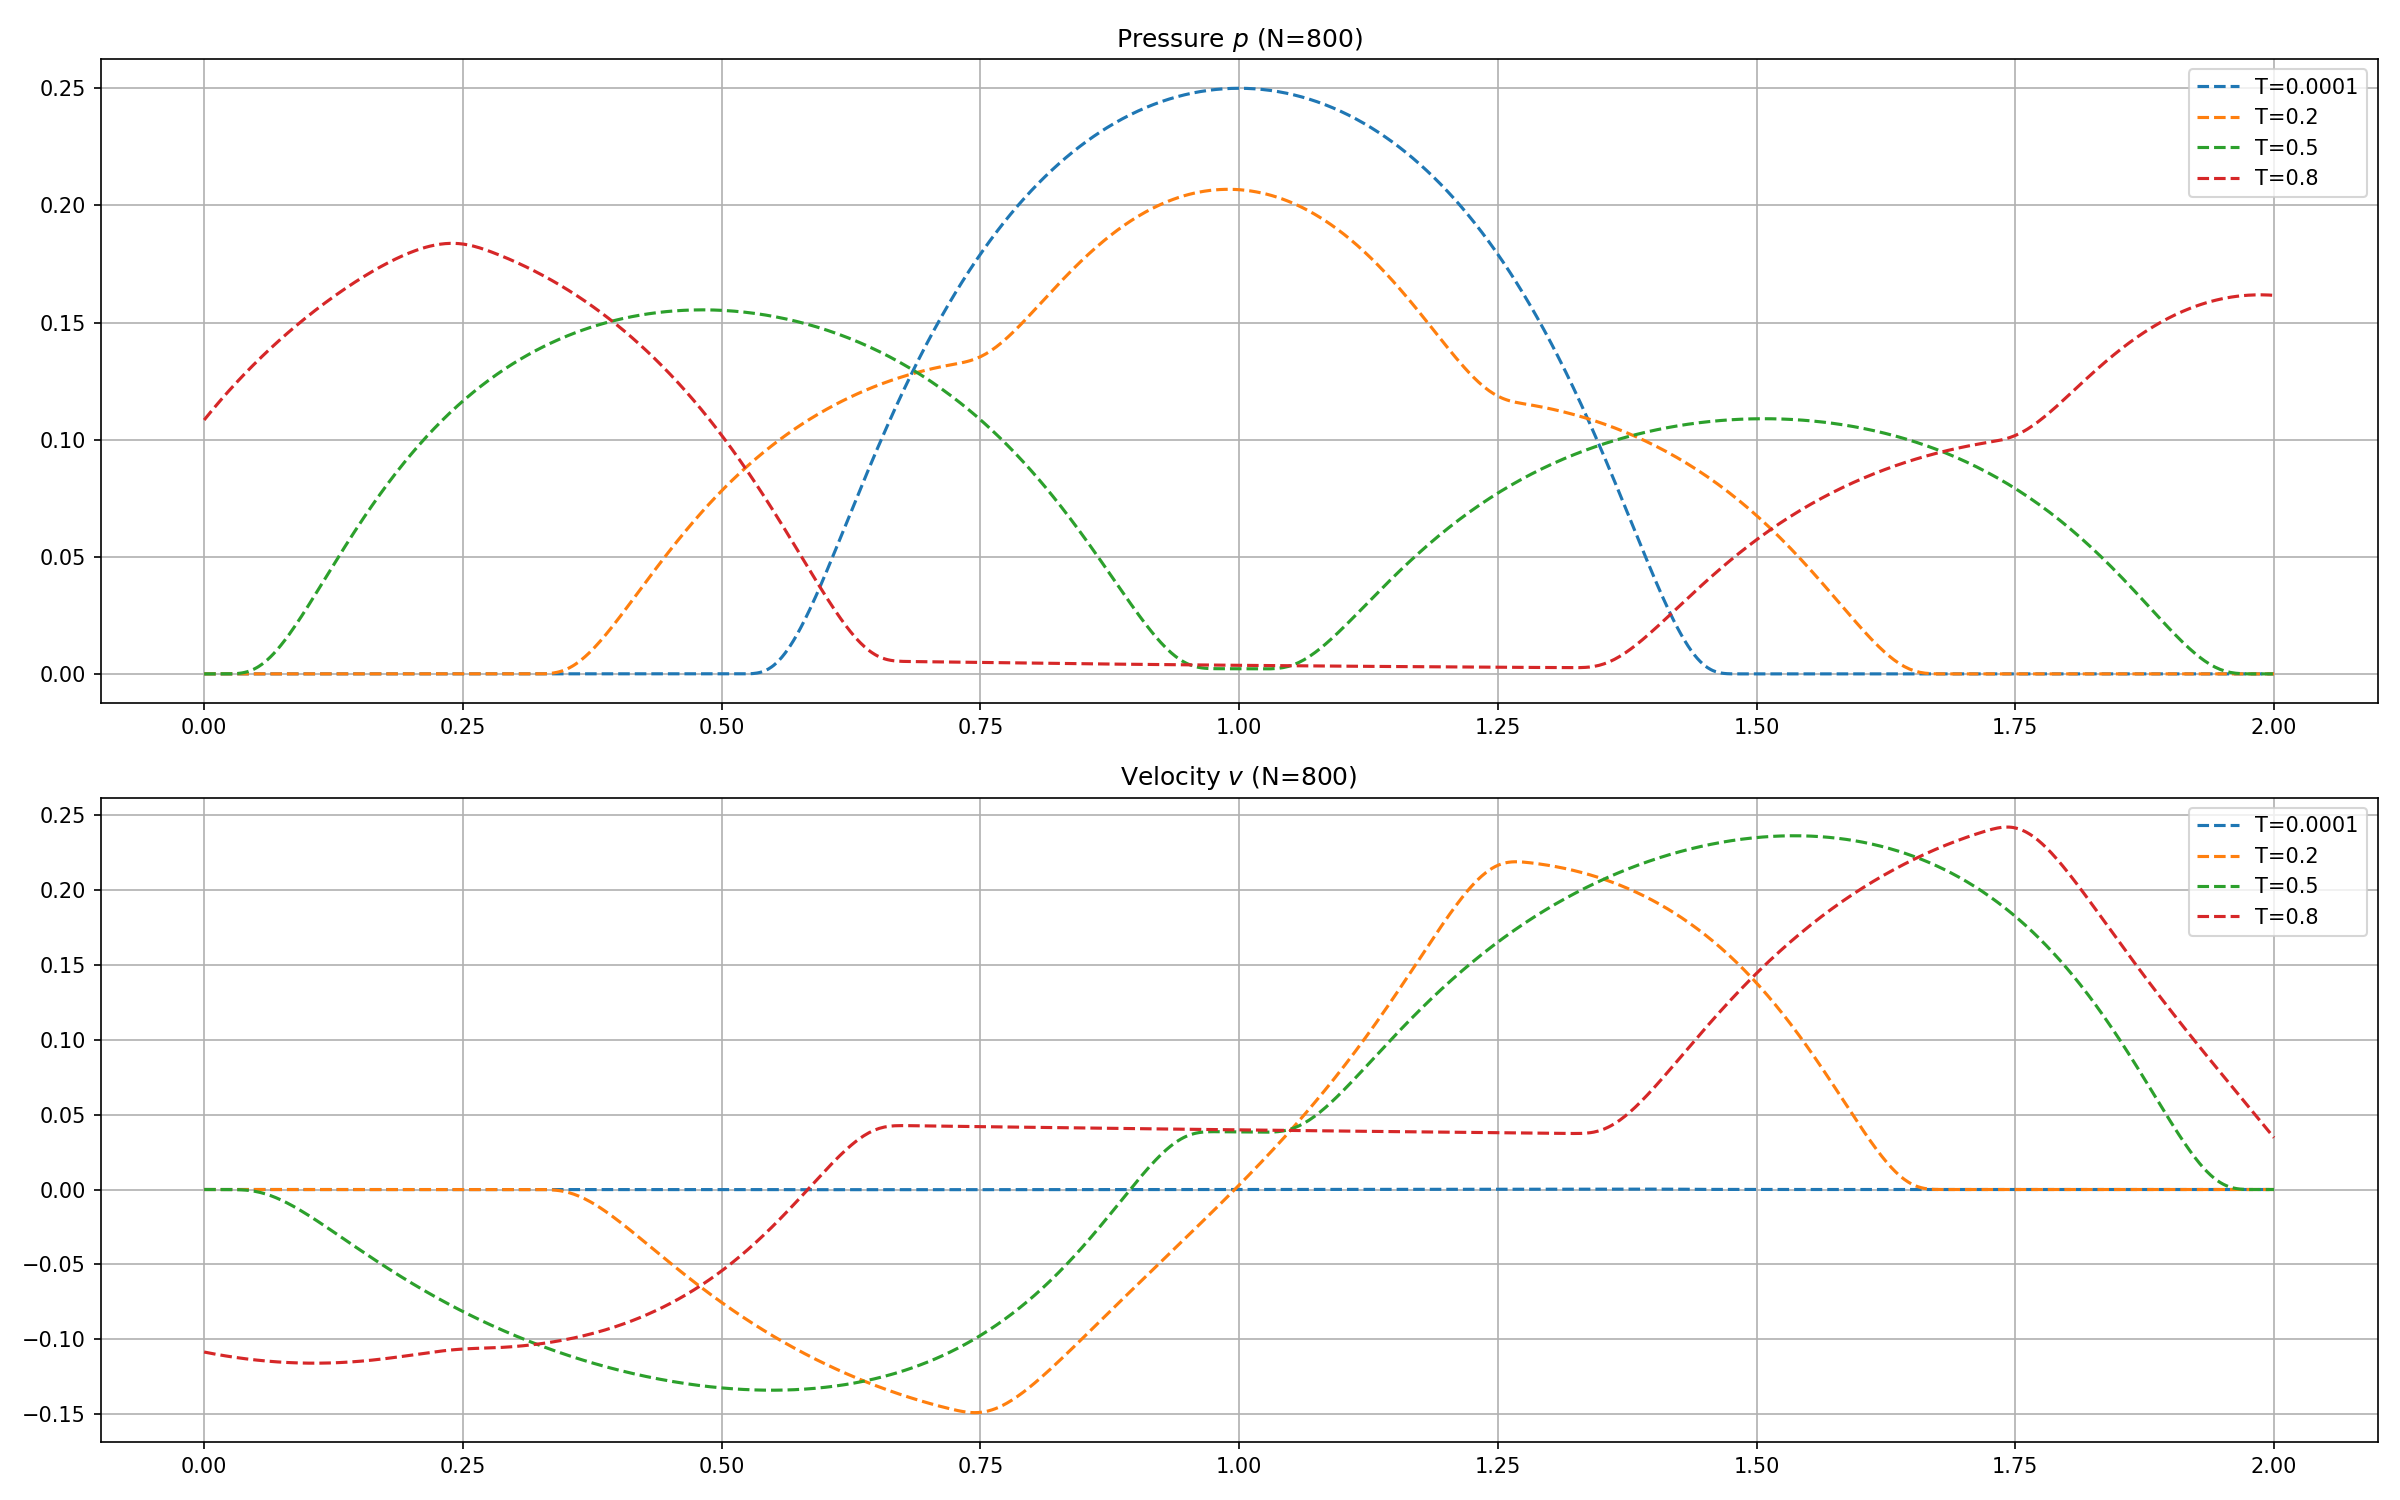
\includegraphics[width=0.9\textwidth]{Images/dg_solution_cone_N800.png}
    \caption{DG numerical solutions cone cross-section.}
    \label{fig:dg_solution_cone}
\end{figure}

The analysis of the numerical results for a non-uniform cross-section is more qualitative due 
to the absence of an analytical solution for direct comparison.
We can oberse that the wave propagation is influenced by the varying cross-sectional area,
as it has stop to be symmetric.
For example, the pressure is amplified in regions where the cross-sectional area decreases. 

\subsection{Performance Study}
A performance study was conducted to evaluate the computational efficiency of the Discontinuous Galerkin Method implementation.
The study focused on measuring the execution time for simulations with varying numbers of elements ($N$). 
\subsubsection{Euler explicit time integration}

\begin{table}[h!]
\centering
\begin{tabular}{c ccc}
\hline
$N \backslash S(x)$ & Const. & Exp. & Cone \\
\hline
100 & 0.250 & 0.154 & 0.142 \\
200 & 0.205 & 0.175 & 0.156 \\
300 & 0.238 & 0.213 & 0.198 \\
400 & 0.325 & 0.249 & 0.245 \\
500 & 0.344 & 0.326 & 0.296 \\
600 & 0.409 & 0.387 & 0.371 \\
700 & 0.569 & 0.545 & 0.522 \\
800 & 0.666 & 0.739 & 0.620 \\
1000 & 1.059 & 1.053 & 1.021 \\
1500 & 2.248 & 2.151 & 2.076 \\
2000 & 3.526 & 3.327 & 3.380 \\
\hline
\end{tabular}
\caption{Execution time (s) of the DG P1 solver using the EULER scheme.}
\label{tab:performance-euler}
\end{table}


\begin{figure}[htbp]
    \centering
    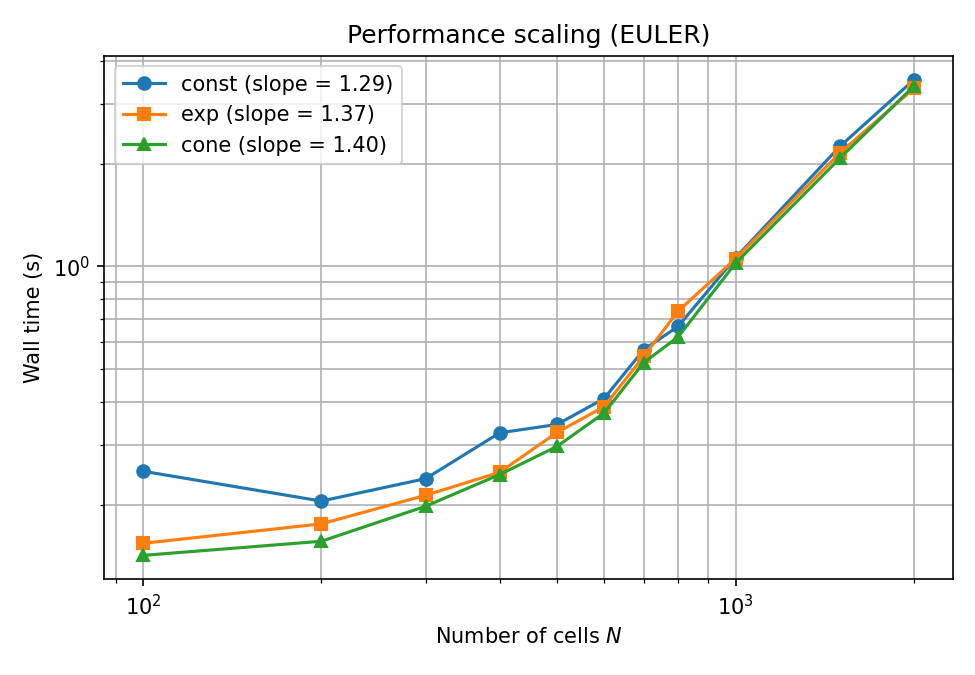
\includegraphics[width=0.7\textwidth]{Images/performance_euler.png}
    \caption{Performance study with Explicit Euler time integration.}
    \label{fig:performance_euler}
\end{figure}

The performance results indicate that the execution time scales under $N^2$. 
Since the performance study was done in JAX framework, the first run includes
compilation time. This explains the higher execution time for the smallest $N$ values 
for the constant cross-section case in \ref{fig:performance_euler}.


\subsubsection{RK2 explicit time integration}

\begin{table}[h!]
\centering
\begin{tabular}{c ccc}
\hline
$N \backslash S(x)$ & Const. & Exp. & Cone \\
\hline
100 & 0.237 & 0.189 & 0.188 \\
200 & 0.325 & 0.218 & 0.225 \\
300 & 0.386 & 0.280 & 0.298 \\
400 & 0.503 & 0.386 & 0.376 \\
500 & 0.594 & 0.502 & 0.487 \\
600 & 0.720 & 0.639 & 0.624 \\
700 & 0.986 & 0.952 & 0.939 \\
800 & 1.205 & 1.162 & 1.173 \\
1000 & 2.079 & 1.943 & 1.962 \\
1500 & 3.931 & 4.024 & 3.937 \\
2000 & 6.579 & 6.484 & 6.693 \\
\hline
\end{tabular}
\caption{Execution time (s) of the DG P1 solver using the RK2 scheme.}
\label{tab:performance-rk2}
\end{table}


\begin{figure}[htbp]
    \centering
    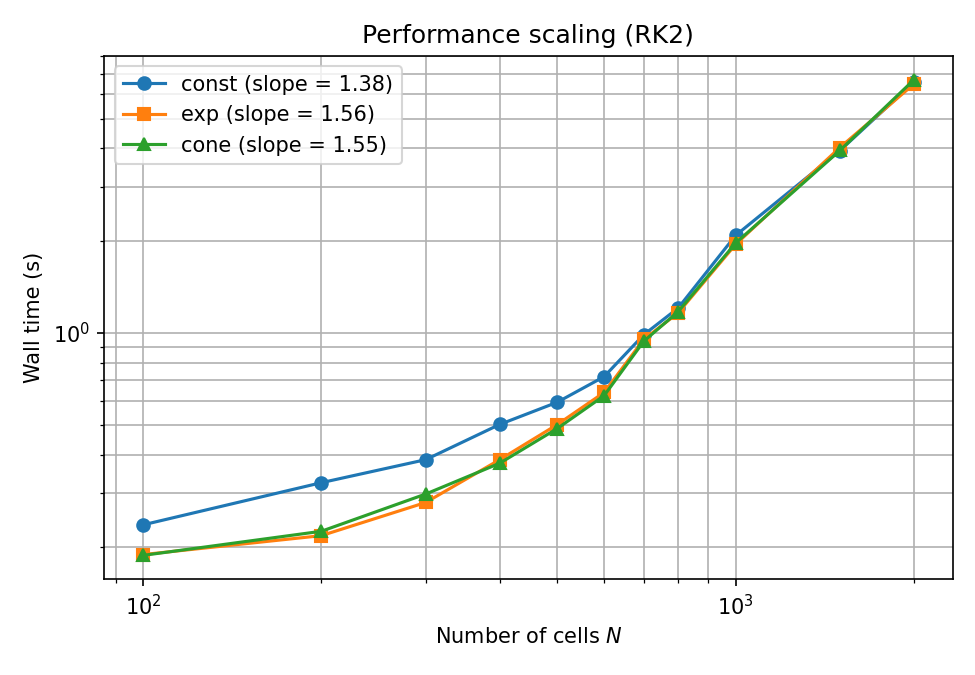
\includegraphics[width=0.7\textwidth]{Images/performance_rk2.png}
    \caption{Performance study with RK2 explicit time integration.}
    \label{fig:performance_rk2}
\end{figure}

The performance results for the RK2 explicit time integration scheme also show a scaling of execution time under $N^2$ 
but superior to the Euler explicit time integration scheme as expected due to the additional computations involved in the RK2 method.
That also explain the higher execution time in the performance study in \ref{tab:performance-rk2}.
 
\newpage
\section{Conclusion}
\newpage
\printbibliography

% Minimal example of an external bibliography (create refs.bib)
% Example BibTeX entry:
%
% @article{doe2020,
%   author = {Doe, John and Example, Anne},
%   title = {Title of the cited article},
%   journal = {Example Journal},
%   year = {2020},
%   volume = {12},
%   pages = {34--56}
% }

\end{document}